%%%%%%%%%%%%%%%%%%%%%%%%%%%%%%%%%%%%%%%
%% NEW CHAPTER
%%%%%%%%%%%%%%%%%%%%%%%%%%%%%%%%%%%%%%%

\chapter{People\clabel{People}}
{\it 
The previous chapter developed a model of individual behaviour based on an
assumed dynamic imposed on wealth. If we know the stochastic process that describes
individual wealth, then we also know what happens at population level -- each individual
is represented by a realisation of the process, and we can compute 
the dynamics of wealth distributions. We answer questions about inequality and poverty in
a model economy which, for the moment, contains no interactions between individuals. We also gain an understanding of when and how results for finite populations differ from those for the infinite ensemble.}
\newpage

%%%%%%%%%%%%%%%%%%%%%%%%%%%%%%%%%%%%%%%

\section{Every man for himself}
\seclabel{Every_man}

We have seen that risk aversion constitutes optimal behaviour under the assumption 
of multiplicative wealth growth and over time scales that are long enough for systematic 
trends to be significant. In this chapter we will continue to explore our null model, 
\GBM. By ``explore'' we mean that we will let the model generate its world -- if 
individual wealth was to follow \GBM, what kind of features of an economy would emerge? 
We will see that cooperation and the formation of social structure also constitute 
optimal behaviour.

\GBM is more than a random variable. It's a stochastic process, either a set of trajectories 
or a family of time-dependent random variables, depending on how we 
prefer to look at it.  Both perspectives are informative in the context of economic modelling:
from the set of trajectories we can judge what is likely to happen to an individual, 
\eg by following a single trajectory for a long time; while the \PDFa of the random 
variable $\x(\t^*)$ at some fixed value of $\t^*$ tells us how wealth is distributed in our model. 

We use the term wealth distribution to refer to the density function, $\PDF_\x(\x)$, and not the process of distributing wealth among people. This can be interpreted as follows. Imagine a population of $\N$ individuals. If I select a random individual, each having uniform probability $\frac{1}{\N}$, then the probability of the selected individual having wealth greater than $\x$ is given by the CDF, $F_\x(\x)=\int_\x^\infty \PDF_\x(s)\gd s$. If $\N$ is large, then $\D \x \PDF_\x(\x)\N$ is the approximate number of individuals who have wealth between $\x$ and $\x+\D \x$. Thus, a broad wealth distribution with heavy tails indicates greater wealth inequality.

\underline{Examples:}
\begin{itemize}
\item Under perfect equality everyone would have the same, meaning that the wealth
distribution would be a Dirac delta function centred at the sample mean of $\x$, that is
\be
\PDF_\x(\x)=\delta(\x-\ave{\x}_\N);
\ee
\item
Maximum inequality would mean that one individual owns everything
and everyone else owns nothing, that is
\be 
\PDF_\x(\x)=\frac{\N-1}{\N}\delta(\x-0)+\frac{1}{\N}\delta(\x-\N\ave{\x}_\N).
\ee
\end{itemize}

%%%%%%%%%%%%%%%%%%%%%%%%%%%%%%%%%%%%%%%

\subsection{Log-normal distribution}
\seclabel{Log-normal_wealth}
At a given time, $\t$, \GBM produces a random variable, $\x(\t)$, with a log-normal distribution whose parameters depend on $\t$. (A log-normally distributed random variable is one whose logarithm is a normally distributed random variable.) If each individual's wealth follows \GBM,
\be
\gd\x=\x(\gmu \gd\t + \gsigma \gd\gW),
\elabel{GBM}
\ee
with solution 
\be
\x(\t) = \x(0) \exp\left[\left(\gmu-\frac{\gsigma^2}{2}\right)\t + \gsigma \gW(\t)\right],
\elabel{GBM_sol}
\ee
then we will observe a log-normal distribution of wealth at each moment in time:
\be
\ln \x(\t) \sim \mathcal{\N}\left(\ln \x(0) + \left(\gmu - \frac{\gsigma^2}{2}\right)\t, \gsigma^2 \t\right).
\elabel{log-normal}
\ee
It will be convenient hereafter to assume the initial condition $\x(0)=1$ (and, therefore, $\ln \x(0)=0$) unless otherwise stated.

Note that the variance of $\ln \x(\t)$ increases linearly in time. We will develop an understanding of this shortly. As we will see, it indicates that any meaningful measure of inequality will grow over time in our simple model. To see what kind of a wealth distribution \eref{log-normal} is, it is worth spelling out the log-normal \PDFa:
\be
\PDF_x(\x)=\frac{1}{\x\sqrt{2\pi \gsigma^2t}}\exp\left(-\frac{[\ln \x-(\gmu-\frac{\gsigma^2}{2})\t]^2}{2\gsigma^2 \t} \right).
\elabel{PDFx}
\ee

This distribution is the subject of a wonderful book \cite{AitchisonBrown1957}, sadly out-of-print now. It will be useful to know some of its basic properties. Of particular importance is the expected wealth under this distribution. This is
\be
\ave{\x(\t)}=\exp(\gmu \t)
\elabel{exp_x}
\ee
or, equivalently, $\ln\ave{\x(\t)}=\gmu \t$. We could confirm this result by calculating $\ave{\x(\t)}=\int_0^\infty s\PDF_\x(s) ds$, but this would be laborious. Instead we use a neat trick, courtesy of \cite[Chapter 4.2]{KloedenPlaten1992}, which will come in handy again in \secref{RGBM_moments}. The idea is to derive from the stochastic differential equation for $\x$, like \eref{GBM}, a solvable ordinary differential equation in the $k^\text{th}$ moment, $\ave{\x^k}$. For the first moment we do this simply by taking expectations of both sides of \eref{GBM}. The noise term vanishes to turn the SDE for $\x$ into an ODE for $\ave{\x}$:
\bea
\ave{\gd\x}&=&\ave{\x(\gmu \gd\t + \gsigma \gd\gW)}\\
d\ave{\x}&=&\ave{\x} \gmu \gd\t + \gsigma \overbrace{\ave{\gd\gW}}^{=0}\\
&=&\ave{\x} \gmu \gd\t.
\eea
This is a very simple first-order linear differential equation, whose solution with initial condition $\x(0)=1$ is given by \eref{exp_x}.

For $\gmu>0$ the expected wealth grows exponentially over time, as do its median and variance:
\bea
\text{median}[\x(\t)] &=& \exp[(\gmu-\gsigma^2/2)\t]; \elabel{median_x} \\
\var[\x(\t)] &=& \exp(2\gmu \t)[\exp(\gsigma^2 \t)-1]. \elabel{var_x}
\eea

%%%%%%%%%%%%%%%%%%%%%%%%%%%%%%%%%%%%%%%

\subsection{Two growth rates}
\seclabel{two_rates}
We will recap briefly here one of our key ideas, covered in detail in \secref{Geometric_Brownian}, that the ensemble average of all possible trajectories of \GBM grows at a different (faster) rate from that achieved by a single trajectory almost surely in the long-time limit. Understanding this difference was the key to developing a coherent theory of individual decision-making. We will see here that it is also crucial in understanding how wealth becomes distributed in a population of individuals whose wealths follow \eref{GBM} and, furthermore, how we can measure the inequality in such a distribution.

We recall from \eref{expectation_g} that the growth rate of the expected wealth is
\be
\gex = \frac{\gd\ln\ave{\x}}{\gd\t} = \gmu,
\ee
and from \eref{time_g} that the time-average growth rate of wealth is
\be
\gt = \frac{\gd\ave{\ln \x}}{\gd\t} = \gmu-\frac{\gsigma^2}{2}.
\ee

%%%%%%%%%%%%%%%%%%%%%%%%%%%%%%%%%%%%%%%

\subsection{Measuring inequality}
\seclabel{Inequality_measure}
In the case of \GBM we have just seen how to 
compute the exact full wealth distribution, $\PDF_\x(\x)$. This is interesting but often we want only summary measures of the distribution. One summary measure of particular interest to economists is inequality. How much inequality is there in a distribution like \eref{log-normal}? And how does this quantity increase over time under \GBM, as we have suggested?

Clearly, to answer these questions, we must quantify ``inequality''. In this section, and also in \cite{AdamouPeters2016}, we develop a natural way of measuring it, which makes use of the two growth rates we identified for the non-ergodic process. We will see that a particular inequality measure, known to economists as Theil's second index of inequality \cite{Theil1967}, is the difference between typical wealth (growing at the time-average growth rate) and average wealth (growing at the ensemble-average growth rate) in our model. Thus, the difference between the time average and ensemble average, the essence of ergodicity breaking, is the fundamental driver of the dynamics of inequality.

The two limits of inequality are easily identified: minimum inequality means that everyone 
has the same wealth, and maximum inequality means that one individual has all the 
wealth and everyone else has nothing. (This assumes that wealth cannot become 
negative.) Quantifying inequality in any other distribution is reminiscent of the gamble 
problem. Recall that for gambles we wanted make statements of the type ``this gamble 
is more desirable than that gamble''. We did this by collapsing a distribution to a 
scalar. Depending on the question that was being asked, 
the appropriate way of collapsing the distribution and the resulting scalar can be different 
(the scalar relevant to an insurance company may not be relevant to an individual). 
In the case of inequality we also have a distribution -- the wealth distribution -- and we 
want to make statements of the type ``this distribution is more unequal than that 
distribution''. Again, this is done by collapsing the distribution to a scalar, and again 
many different choices of collapse and resulting scalar are possible. The Gini 
coefficient is a particularly well-known scalar of this type, the 80/20 ratio another. Indeed, there is a whole menagerie of inequality measures.

In this context the expectation value is an important quantity. 
For instance, if everyone has the same wealth, then everyone will own the average, $\x_\gi=\ave{\x}_\N$, which converges to the expectation value for large $\N$. Also, whatever the distribution 
of wealth, the total wealth is $\N\ave{\x}_\N$ which converges to $\N\ave{\x}$ as $\N$ grows large. The growth 
rate of the expectation value, $\gex$, thus tells us how fast the average wealth and the 
total population wealth grow with probability one in a large ensemble. The time-average growth rate, $\gt$, on the other hand, tells us how fast an individual's wealth grows almost surely in 
the long run. If the typical individual's wealth grows more slowly than the 
expectation value of wealth, then there must be atypical individuals with very large 
wealths to account for the difference. This insight suggests the following measure of 
inequality.

\definition{
Inequality, $J$, is the quantity whose growth rate is the 
difference between expectation-value and time-average growth rates,
\be
\frac{\gd J}{\gd\t}=\gex-\gt.
\elabel{dJ}
\ee
\Eref{dJ} defines the dynamic of inequality, and inequality itself is found by 
integrating over time:
\be
J(\t)=\int_0^\t \gd s [\gex(s)-\gt(s)].
\elabel{J}
\ee
}

This definition may be used for dynamics other than
\GBM, as we shall discuss in \secref{jensen}. Whatever the wealth dynamic, typical minus average growth rates are informative of the
dynamic of inequality. Within the \GBM framework we can write the difference in growth rates as 
\be
\frac{\gd J}{\gd\t}=\frac{\gd \ln \ave{\x}}{\gd\t}-\frac{\gd \ave{\ln \x}}{\gd\t}
\elabel{J_dyn}
\ee
and integrate over time to get
\be
J(\t)=\ln \ave{\x(\t)}-\ave{\ln \x(\t)}.
\elabel{J_x}
\ee
This quantity is known as the mean logarithmic deviation (MLD) or Theil's second index of inequality \cite{Theil1967}. 
This is rather remarkable. Our general inequality measure, \eref{J}, evaluated 
for the specific case of \GBM, turns out to be a well-known measure of inequality that 
economists have identified independently, without considering non-ergodicity and ensemble 
average and time average growth rates. Merely by insisting on measuring inequality well,
Theil used the \GBM model implicitly.\footnote{Like Kelly's ideas about gambling \cite{Kelly1956}, Theil's inequality measures were developed using information theory.}

Substituting the known values of the two growth rates into \eref{dJ} and integrating, we can evaluate the Theil inequality as a function of time:
\be
J(\t)=\frac{\gsigma^2}{2} \t.
\elabel{J_t}
\ee
Thus we see that, in \GBM, our measure of inequality increases indefinitely.

%%%%%%%%%%%%%%%%%%%%%%%%%%%%%%%%%%%%%%%

\subsection{Wealth condensation}
\seclabel{condensation}
The log-normal distribution generated by \GBM broadens indefinitely, \eref{var_x}. Likewise, the inequality present in the distribution -- measured as the time-integrated difference between ensemble and time average growth rates -- grows without bound. A related property of \GBM is the evolution towards wealth condensation. Wealth condensation means that a single individual will own a non-zero fraction of the total wealth in the population in the limit of large $\N$, see \eg \cite{BouchaudMezard2000}. In the present case an arbitrarily large share ofthe  total wealth will be owned by an arbitrarily small share of the population.

One simple way of seeing this is to calculate the fraction of the population whose wealths are less than the expected wealth, \ie $\x(\t)<\exp(\gmu \t)$. To do this, we define a new random variable, $z(\t)$, whose distribution is the standard normal:
\be
z(\t) \equiv \frac{\ln \x(\t) - (\gmu-\gsigma^2/2)\t}{\gsigma \t^{1/2}} \sim \mathcal{\N}(0,1).
\ee
We want to know the mass of the distribution with $\ln \x(\t)<\gmu \t$. This is equivalent to $z<\gsigma \t^{1/2}/2$, so the fraction below the expected wealth is
\be
\Phi\left(\frac{\gsigma \t^{1/2}}{2}\right),
\ee
where $\Phi$ is the CDF of the standard normal distribution. This increases over time, tending to one as $\t\to\infty$.

%%%%%%%%%%%%%%%%%%%%%%%%%%%%%%%%%%%%%%%

\subsection{Rescaled wealth}
\seclabel{rescaled}
Economists have arrived at many inequality measures, and have drawn up a list of conditions that particularly useful measures of inequality satisfy. Such measures are called ``relative measures'' \cite[Appendix 4]{Sen1997} and $J$ is one of them.

One of the conditions is that inequality measures should not change when $\x$ is divided by the same factor for everyone. Since we are primarily interested in inequality in this section, we can remove absolute wealth levels from the analysis and study an object called the rescaled wealth.

\definition{
The rescaled wealth, 
\be
y_\gi(\t) = \frac{\x(\t)}{\ave{\x(\t)}_\N},
\elabel{rescaled}
\ee
is the proportion of the sample mean wealth -- \ie the wealth averaged over the finite population -- owned by an individual.}

This quantity is useful because its numerical value does not 
depend on the currency used: it is a dimensionless number. 
Thus if my rescaled wealth is $y_\gi(\t) = 1/2$, it means that my wealth is half the 
average wealth, irrespective of whether I measure it in Kazakhstani Tenge 
or in Swiss Francs. The sample mean rescaled wealth is easily calculated:
\be
\ave{y_\gi(\t)}_\N = \ave{\frac{\x(\t)}{\ave{\x(\t)}_\N}}_\N = 1.
\ee

If the population size, $\N$, is large enough, then we might expect the sample mean wealth, $\ave{\x(\t)}_\N$, to be close to the ensemble average, $\ave{\x(\t)}$, which is simply its $\N\to\infty$ limit. We will discuss more carefully when this approximation holds for wealths following \GBM in \secref{finite_populations}. Let's assume for now that it does. The rescaled wealth is then well approximated as
\be
y_\gi(\t) = \frac{\x_\gi(\t)}{\ave{\x(\t)}} = \x_\gi(\t)\exp(-\gmu \t).
\ee

Now that we have an expression for $y$ in terms of $\x$ and $\t$, we can derive the dynamic for rescaled wealth using \Ito's formula (just as we did to find the wealth dynamic for a general utility function in \secref{dyn_from_u}). We start with
\bea
\gd y &=& \frac{\partial y}{\partial \t}\gd\t + \frac{\partial y}{\partial \x}\gd\x + \frac{1}{2} \frac{\partial^2 y}{\partial \x^2} \gd\x^2 \\
&=& -\gmu y\gd\t + \frac{y}{\x}\gd\x \elabel{ysde},
\eea
and then substitute \eref{GBM} for $\gd\x$ to get
\be
\gd y = y \gsigma \gd\gW.
\elabel{GBM_y}
\ee
So $y(\t)$ follows a very simple \GBM with zero drift and volatility $\gsigma$. This means that rescaled wealth, like wealth, has an ever-broadening log-normal distribution:
\be
\ln y(\t) \sim \mathcal{\N}\left(-\frac{\gsigma^2}{2}\t, \gsigma^2 \t\right).
\elabel{log-normal_y}
\ee

Finally, noting that $\ave{\ln y}=\ave{\ln \x}-\ln\ave{\x}$ gives us a simple expression for our inequality measure in \eref{J_x} in terms of the rescaled wealth:
\be
J(\t)=-\ave{\ln y}.
\ee

%%%%%%%%%%%%%%%%%%%%%%%%%%%%%%%%%%%%%%%

\subsection{$u$-normal distributions and Jensen's inequality}
\seclabel{jensen}
So far we have confined our analysis to \GBM, where wealths follow the dynamic specific by \eref{GBM}. However, as we discussed in the context of gambles, other wealth dynamics are possible. In particular, we explored the dynamics corresponding to invertible utility functions, where utility executes a \BM with drift as in \eref{bm_u}:
\be
\gd\gu = a_\gu \gd\t + b_\gu \gd\gW.
\ee
Under this dynamic, utility is normally distributed,
\be
u(\x(\t)) \sim \mathcal{\N}\left(a_u\t, {b_u}^2 \t\right),
\ee
and we can say that wealth has a ``$\gu$-normal'' distribution. For \GBM, the corresponding utility function is, as we know, $u(\x)=\ln \x$, and $\gu$-normal becomes log-normal.

Replacing the logarithm in \eref{J_x} by the general utility function gives a general expression for our wealth inequality measure,
\be
J_\gu(\t)=\gu(\ave{\x(\t)}) - \ave{\gu(\x(\t))}.
\elabel{J_u}
\ee
It's not easy to write a general expression for $J_\gu(\t)$ in only $\t$ and the model parameters $a_\gu$ and $b_\gu$, because it would involve the solution of the general wealth dynamic in \eref{dx}. However, we can still say something about how inequality evolves. Let's see what happens if we start with perfect equality, $\x_\gi(0)=\x_0$ with $\x_0$ fixed, and then let wealths evolve a little to $\x(\D \t)=\x_0+\D \x$, where $\D \x$ is a random wealth increment generated by the wealth dynamic. The change in inequality would be
\be
\D J_\gu = \gu(\ave{\x_0+\D \x}) - \ave{\gu(\x_0+\D \x)},
\ee
since $\gu(\ave{\x_0})=\ave{\gu(\x_0)}=\gu(\x_0)$.

We can now appeal to Jensen's inequality: if $\gu$ is a concave function, like the logarithm, then $\D J_\gu \geq 0$; while if $\gu$ is convex, like the curious exponential in \eref{test_dyn_u}, then $\D J_\gu \leq 0$. The only cases for which $\D J_\gu=0$ are if $\D \x$ is non-random or if $\gu$ is linear. Thus, it is both randomness and the nonlinearity of the utility function -- or ergodicity transformation, if we make that equivalence -- that creates a difference in growth rates and generates inequality.

%%%%%%%%%%%%%%%%%%%%%%%%%%%%%%%%%%%%%%%

\subsection{power-law resemblance}
\seclabel{power_law}
It is an established empirical observation \cite{Newman2005} that the upper tails of 
real wealth distributions look more like a power-law than a log-normal. Our trivial model does not
strictly reproduce this feature, but it is instructive to compare the log-normal distribution
to a power-law distribution. A power-law \PDFa has the asymptotic form 
\be
\PDF_\x(\x)= \x^{-\alpha},
\elabel{power_law}
\ee
for large arguments $\x$. This implies that the logarithm of the \PDFa is proportional 
to the logarithm of its argument, $\ln \PDF_\x(\x) = -\alpha \ln \x$. Plotting
one against the other will yield a straight line, the slope being the exponent $-\alpha$. 

Determining whether an empirical observation is consistent with such behaviour 
is difficult because the behaviour to be observed is in the tail (large $\x$) where data are,
by definition, sparse. A quick-and-dirty way of checking for possible power-law 
behaviour is to plot an empirical \PDFa against its argument on log-log scales, 
look for a straight line, and measure the slope. However, plotting any distribution on any 
type of scales results in some line. It may not be a straight line but it will have some slope 
everywhere. For a known distribution (power-law or not) we can interpret this slope 
as a local apparent power-law exponent. 

What is the local apparent power-law exponent of a log-normal wealth distribution near the 
expectation value $\ave{\x}=\exp(\gmu \t)$, \ie in the upper tail where approximate power-law behaviour
has been observed empirically? The logarithm of \eref{PDFx} is
\bea
\ln \PDF(\x) =& -\ln\left(\x\sqrt{2\pi \gsigma^2t}\right) -\frac{[\ln \x-(\gmu-\frac{\gsigma^2}{2})\t]^2}{2\gsigma^2 \t}\\
=& -\ln \x -\frac{\ln (2\pi \gsigma^2t)}{2} - \frac{(\ln \x)^2-2(\gmu-\frac{\gsigma^2}{2})\t \ln \x+(\gmu-\frac{\gsigma^2}{2})^2t^2}{2\gsigma^2 \t}.
\eea
Collecting terms in powers of $\ln \x$ we find
\be
\ln \PDF(\x)=-\frac{(\ln \x)^2}{2\gsigma^2 \t}  + \left(\frac{\gmu}{\gsigma^2}-\frac{3}{2}\right)\ln \x - \frac{\ln(2 \pi\gsigma^2 \t)}{2}-\frac{(\gmu-\frac{\gsigma^2}{2})^2t}{2\gsigma^2}
\ee
with local slope, \ie apparent exponent,
\be
\frac{\gd\ln \PDF(\x)}{\gd \ln \x} = - \frac{\ln \x}{\gsigma^2 \t}  + \frac{\gmu}{\gsigma^2} - \frac{3}{2}.
\ee
Near $\ave{\x}$, $\ln \x \sim \gmu \t$ so that the first two terms cancel approximately. Here the distribution will resemble a power-law with exponent $-3/2$ when plotted on doubly logarithmic scales. (The distribution will also look like a power-law where the first term is much smaller than the others, \eg where $\ln \x \ll \gsigma^2 \t$.) We don't believe that such empirically observed power-laws are merely a manifestation of this mathematical feature. Important real-world  mechanisms that broaden real wealth distributions, \ie concentrate wealth, are missing from the null model. However, it is interesting that the trivial model of \GBM reproduces so many qualitative features of empirical observations. 

%%%%%%%%%%%%%%%%%%%%%%%%%%%%%%%%%%%%%%%

\section{Finite populations}
\seclabel{finite_populations}
So far we have considered the properties of the random variable, $\x(\t)$, generated by \GBM at a fixed time, $\t$. Most of the mathematical objects we have discussed are, strictly speaking, relevant only in the limit $\N\to\infty$, where $\N$ is the number of realisations of this random variable. For example, the expected wealth, $\ave{\x(\t)}$, is the limit of the sample mean wealth
\be
\ave{\x(\t)}_\N \equiv \frac{1}{\N}\sum_{i=1}^\N \x_\gi(\t),
\elabel{sample}
\ee
as the sample size, $\N$, grows large. In reality, human populations can be very large, say $\N\sim10^7$ for a nation state, but they are most certainly finite. Therefore, we need to be diligent and ask what the effects of this finiteness are. In particular, we will focus on the sample mean wealth under \GBM. For what values of $\gmu$, $\gsigma$, $\t$, and $\N$ is this well approximated by the expectation value? And when it is not, what does it resemble?

\subsection{Sums of log-normals}
\seclabel{sketch}
In \cite{PetersKlein2013} we studied the sample mean of \GBM, which we termed the ``partial ensemble average'' (PEA). This is the average of $\N$ independent realisations of the random variable $\x(\t)$, \eref{sample}. Here we sketch out some simple arguments about how this object depends on $\N$ and $\t$.

Considering the two growth rates in \secref{two_rates}, we anticipate the following tension:
\begin{enumerate}
\item[A)] for large $\N$, the PEA should resemble the expectation value, $\exp(\gmu \t)$;
\item[B)] for long $\t$, all trajectories in the sample -- and, therefore, the sample mean itself -- should grow like $\exp[(\gmu-\gsigma^2/2)\t]$.
\end{enumerate}
Situation A -- when a sample mean resembles the corresponding expectation value -- is known in statistical physics as ``self-averaging.'' A simple strategy for estimating when this occurs is to look at the relative variance of the PEA,
\be
R \equiv \frac{\var[\ave{\x(\t)}_\N]}{\ave{\ave{\x(\t)}_\N}^2}.
\elabel{rel_var}
\ee
To be explicit, here the $\ave{\cdot}$ and $\text{var}(\cdot)$ operators, 
without $\N$ as a subscript, 
refer to the mean and variance over all possible PEAs. The PEAs themselves, taken over finite samples of size $\N$, are denoted $\ave{\cdot}_\N$. \Eref{rel_var} simplifies to
\be
R = \frac{\frac{1}{\N}\var[\x(\t)]}{\ave{\x(\t)}^2},
\ee
into which we insert \eref{exp_x} and \eref{var_x} to get an expression in terms of the \GBM model parameters:
\be
R = \frac{e^{\gsigma^2 \t}-1}{\N}.
\elabel{rel_var_N}
\ee
If $R \ll 1$, then the PEA will likely be close to its own expectation value, which is equal to the expectation value of the \GBM. Therefore, $\ave{\x(\t)}_\N\approx\ave{\x(\t)}$ when
\be
\t < \frac{\ln \N}{\gsigma^2}.
\elabel{short_t}
\ee
This hand-waving tells us roughly when the large-sample -- or, as we see from \eref{short_t}, short-time or low-volatility -- self-averaging regime holds. A more careful estimate of the cross-over time in \eref{t_c} is a factor of 2 larger, as we shall see in \secref{REM}, but the scaling is identical.

For $\t>\ln \N/\gsigma^2$, the growth rate of the PEA transitions from $\gmu$ to its $\t\to\infty$ limit of $\gmu-\gsigma^2/2$ (Situation B). 
Another way of viewing this is to think about what dominates the average. For early times in the process, all trajectories are close together and none dominate the PEA. However, as time goes by the distribution broadens exponentially. Since each trajectory contributes with the same weight to the PEA, after some time the PEA will be dominated by the maximum in the sample,
\be
\ave{\x(\t)}_\N \approx \frac{1}{\N}\max_{\gi=1}^\N \{\x_\gi(\t)\}.
\ee
All of these features are illustrated in \fref{trajectories}.

Self-averaging stops when even the ``luckiest'' trajectory is no longer close to the expectation value $\exp(\gmu \t)$. This is guaranteed to happen eventually because the probability for a trajectory to reach $\exp(\gmu \t)$ decreases towards zero as $\t$ grows, as we saw in \secref{condensation}. Naturally, this takes longer for larger samples, which have more chances to contain a lucky trajectory. 

\begin{figure}
\centering
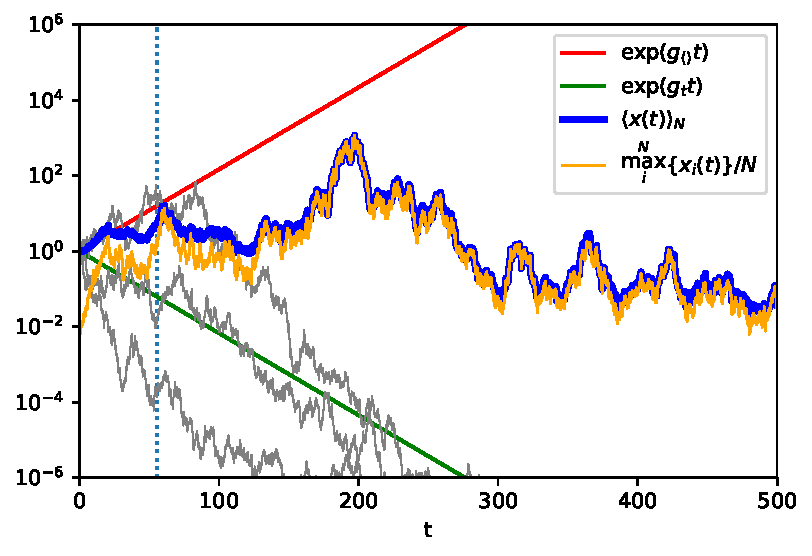
\includegraphics[height=9.3cm]{./chapter_people/figs/trajectories.pdf}
\caption{PEA and maximum in a finite ensemble of size $\N=256$. {\bf \underline{Red line:}} expectation value $\ave{\x(\t)}$. 
{\bf \underline{Green line:}} exponential growth at the time-average growth rate. In the $\t\to\infty$ limit all trajectories grow at this rate. 
{\bf \underline{Yellow line:}} contribution of the maximum value of any trajectory at time $\t$ to the PEA.  
{\bf \underline{Blue line:}} PEA $\ave{\x(\t)}_\N$.
{\bf \underline{Vertical line:}} Crossover -- for $\t>\t_c=\frac{2\ln \N}{\gsigma^2}$ the maximum begins to dominate the PEA (the yellow line approaches the blue line).
{\bf \underline{Grey lines:}} randomly chosen trajectories -- any typical trajectory soon grows at the time-average growth rate.  
{\bf \underline{Parameters:}} $\N=256$, $\gmu=0.05$, $\gsigma=\sqrt{0.2}$.}
\flabel{trajectories}
\end{figure}
\FloatBarrier

In \cite{PetersKlein2013} we analysed PEAs of \GBM analytically and numerically. Using \eref{GBM_sol} the PEA can be written as
\be
\ave{\x}_\N=\frac{1}{\N} \sum_{i=1}^\N \exp\left[ \left(\gmu-\frac{\gsigma^2}{2}\right) \t + \gsigma \gW_i(\t) \right],
\elabel{PEA}
\ee
where $\left\{\gW_i(\t)\right\}_{i=1\dots \N}$ are $\N$ independent realisations of the Wiener process. Taking the deterministic part out of the sum, we can write
\be
\ave{\x}_\N=\exp\left[ \left(\gmu-\frac{\gsigma^2}{2}\right) \t \right] \frac{1}{\N} \sum_{i=1}^\N \exp\left(\t^{1/2} \gsigma \xi_i\right),
\elabel{PEA_2}
\ee
where $\left\{\xi_i\right\}_{i=1\dots \N}$ are $\N$ independent standard normal variates.

We found that typical trajectories of PEAs grow at $\gex$ up to a time $t_c$ 
that is logarithmic in $\N$, meaning $\t_c\propto \ln \N$. This is consistent with our analytical sketch. After this time, typical 
PEA trajectories begin to deviate from expectation-value behaviour, and eventually 
their growth rate converges to $g_t$. While the two limiting behaviours $\N\to\infty$
and $\t\to \infty$ can be computed exactly, what happens in between
is less straightforward. The PEA is a random object outside these limits. 

A quantity of crucial interest to us is the exponential growth rate experienced by the PEA, 
\be
\gest(\t,\N) \equiv \frac{\ln(\ave{\x(\t)}_\N)- \ln(\x(0))}{\t-0} = \frac{1}{\t}\ln(\ave{\x(\t)}_\N).
\elabel{g_est}
\ee
In \cite{PetersKlein2013} we proved that the $\t\to\infty$ limit for any (finite) 
$\N$ is the same as for the case $\N=1$, 
\be
\lim_{\t\to\infty}\gest(\t,\N)=\gmu-\frac{\gsigma^2}{2}
\elabel{gest_2}
\ee
for all $\N\geq1$. Substituting \eref{PEA_2} in \eref{g_est} produces
\bea
\gest(\t,\N)&=&\gmu-\frac{\gsigma^2}{2}+\frac{1}{\t} \ln\left(\frac{1}{\N} \sum_{i=1}^\N \exp( \t^{1/2} \gsigma \xi_i)\right)\\
&=&\gmu-\frac{\gsigma^2}{2}-\frac{\ln \N}{\t}+\frac{1}{\t} \ln\left(\sum_{i=1}^\N \exp( \t^{1/2} \gsigma \xi_i)\right).
\elabel{gest_4}
\eea

We didn't look in \cite{PetersKlein2013} at the expectation value of $\gest(\t,\N)$ for finite time and finite samples, but it's an interesting object that depends on $\N$ and $\t$ but is not stochastic. Note that this is not $\gest$ of the expectation value, 
which would be the $\N\to\infty$ limit of \eref{g_est}. Instead it is the 
$S\to\infty$ limit,
\be
\ave{\gest(\t,\N)} = \frac{1}{\t}\ave{\ln(\ave{\x(\t)}_\N)} = f(\N,\t),
\elabel{gest_3}
\ee
where, as previously, $\ave{\cdot}$ without subscript refers to the average over all possible samples, \ie $\lim_{S\to\infty}\ave{\cdot}_{S}$. The last two terms in \eref{gest_4} suggest an exponential relationship between ensemble size and time. The final term is a tricky stochastic object on which the properties of the expectation value in \eref{gest_3} will hinge. This term will be the focus of our attention: the sum of exponentials of normal random variates or, equivalently, log-normal variates.

\subsection{The random energy model}
\seclabel{REM}
Since the publication of \cite{PetersKlein2013} we have learned, thanks to discussions with J.-P.~Bouchaud, 
that the key object in \eref{gest_4} -- the sum log-normal random variates -- has been of
interest to the mathematical physics community since the 1980s. The reason for this is Derrida's random energy model \cite{Derrida1980,Derrida1981}, which we will describe here. This section is very ``physicsy'' and the key results are in \eref{gest_7} and \eref{gest_8} -- it's safe to skip to them, if you like.

The model is defined as follows. Imagine a system whose energy levels are $2^K=\N$ normally-distributed random numbers, $\xi_i$ (corresponding to $K$ spins). This is a very simple model of a disordered system, such as a spin glass, the idea being that the system is so complicated that we ``give up'' and simply model its energy levels as realisations of a random variable. (We denote the number 
of spins by $K$ and the number of resulting energy levels by $\N$, while Derrida uses $\N$ for the number of spins). The partition function is then
\be
Z=\sum_{\gi=1}^\N \exp\left(\beta J\sqrt{\frac{K}{2}}\xi_\gi\right),
\elabel{Z}
\ee
where the inverse temperature, $\beta$, is measured in appropriate units, and the scaling in $K$ is chosen
so as to ensure an extensive thermodynamic limit \cite[p.~79]{Derrida1980}. $J$ is a constant that will be determined below.
The logarithm of the partition function gives the Helmholtz free energy, 
\bea
F&=&-\frac{\ln Z}{\beta}\\
&=&-\frac{1}{\beta}  \ln\left[\sum_{\gi=1}^\N \exp\left(\beta J \sqrt{\frac{K}{2}}\xi_\gi\right)\right].
\elabel{F}
\eea

Like the growth rate estimator in \eref{g_est}, this involves a sum of 
log-normal variates and, indeed, we can rewrite \eref{gest_4} as
\be
\gest=\gmu-\frac{\gsigma^2}{2}-\frac{\ln \N}{\t}-\frac{\beta F}{\t},
\elabel{gest_5}
\ee
which is valid provided that
\be
\beta J \sqrt{\frac{K}{2}}=\gsigma \t^{1/2}.
\elabel{map}
\ee
\Eref{map} does not give a unique mapping between the parameters of our \GBM, $(\gsigma, \t)$, and the parameters of the REM, $(\beta, K, J)$. Equating (up to multiplication) the constant parameters, $\gsigma$ and $J$, in each model gives us a specific mapping:
\be
\gsigma=\frac{J}{\sqrt{2}} \quad \text{and} \quad \t^{1/2} = \beta\sqrt{K}.
\elabel{choice_1}
\ee

The expectation value of $\gest$ is interesting. The only random object
in \eref{gest_5} is $F$. Knowing $\ave{F}$ thus amounts to knowing $\ave{\gest}$.
In the statistical mechanics of the random energy model, $\ave{F}$ is of key
interest and so much about it is known. We can use this knowledge
thanks to the mapping between the two problems.

Derrida identifies a critical temperature,
\be
\frac{1}{\beta_c} \equiv \frac{J}{2\sqrt{\ln 2}},
\elabel{beta_c}
\ee
above and below which the expected free energy scales differently with $K$ and $\beta$. This maps to a critical time scale in \GBM,
\be
\t_c = \frac{2\ln \N}{\gsigma^2},
\elabel{t_c}
\ee
with high temperature ($1/\beta>1/\beta_c$) corresponding to short time ($\t<\t_c$) and low temperature ($1/\beta<1/\beta_c$) corresponding to long time ($\t>\t_c$). Note that $t_c$ in \eref{t_c} scales identically with $\N$ and $\gsigma$ as the transition time, \eref{short_t}, in our sketch.

In \cite{Derrida1980}, $\ave{F}$ is computed in the high-temperature (short-time) regime as
\bea
\ave{F}&=&E-S/\beta \\
&=&-\frac{K}{\beta} \ln2 - \frac{\beta K J^2}{4},
\elabel{F_2}
\eea
and in the low-temperatures (long-time) regime as
\be
\ave{F}=-KJ\sqrt{\ln 2}.
\elabel{F_3}
\ee

\paragraph{\underline{Short time}}
\mbox{}

We look at the short-time behavior first (high $1/\beta$, \eref{F_2}).
The relevant computation of the entropy $S$ in \cite{Derrida1980} 
involves replacing the number of energy levels
$\N(E)$ by its expectation value $\ave{\N(E)}$. This is justified because
the standard deviation of this number is $\sqrt{\N}$ and relatively small
when $\ave{\N(E)}>1$, which is the interesting regime in Derrida's case. 

For spin glasses, the expectation value of $F$ is interesting, supposedly, 
because the system may be self-averaging and can be thought of as an
ensemble of many 
smaller sub-systems that are essentially independent. The macroscopic
behavior is then given by the expectation value.

Taking expectation values and substituting from \eref{F_2} in \eref{gest_5} we find
\be
\ave{\gest}^{\text{short}}=\gmu-\frac{\gsigma^2}{2}+\frac{1}{\t} \frac{K J^2}{4T^2}.
\elabel{gest_6}
\ee
From \eref{map} we know that $\t=\frac{KJ^2}{2\gsigma^2T^2}$, which we substitute to find
\be
\ave{\gest}^{\text{short}}=\gmu.
\elabel{gest_7}
\ee
This is the correct behavior in the short-time regime.

\paragraph{\underline{Long time}}
\mbox{}

Next, we turn to the expression for the long-time regime (low temperature, \eref{F_3}). 
Again 
taking expectation values and substituting, this time from \eref{F_3} in \eref{gest_5}, we find
for long times
\be
\ave{\gest}^{\text{long}}=\gmu-\frac{\gsigma^2}{2}-\frac{\ln{\N}}{\t}+\sqrt{\frac{2\ln \N}{\t}}\,\gsigma,
\elabel{gest_8}
\ee
which has the correct long-time asymptotic behavior.
The form of the correction to the time-average growth rate
in \eref{gest_8} is consistent with \cite{PetersKlein2013} and \cite{Redner1990}, where
it was found that approximately $\N=\exp(\t)$ systems are required for ensemble-average
behavior to be observed for a time $\t$, so that the parameter $\ln \N/\t$ controls
which regime dominates. If the parameter is small, then \eref{gest_8} indicates that the
long-time regime is relevant.

\Fref{1} is a direct comparison between the results derived
here, based on \cite{Derrida1980}, and numerical results using the same parameter 
values as in \cite{PetersKlein2013}, namely $\gmu=0.05, \gsigma=\sqrt{0.2}, \N=256$ and $S=10^5$.

Notice that $\ave{\gest}$ is not the (local)
time derivative $\frac{\partial}{\partial \t}\ave{\ln(\ave{\x}_\N)}$, but a time-average growth rate, $\ave{\frac{1}{\t}\ln\left( \frac{\ave{\x(\t)}_\N}{\ave{\x(0)}_\N}\right)}$. It is remarkable that the expectation value $\ave{\gest(\N,\t)}$ so closely reflects the
median, $q_{0.5}$, of $\ave{\x}_\N$, \ie
\be
q_{0.5}(\ave{\x(\t)}_\N) \approx \exp \left(\ave{\gest(\N,\t)}\t\right).
\elabel{quant_ave}
\ee
In \cite{PetersGell-Mann2016} it was discussed in detail that 
$\gest(1,\t)$ is an ergodic observable for \eref{GBM}, in the sense that 
$\ave{\gest(1,\t)}=\lim_{\t\to\infty} \gest$. The relationship in \eref{quant_ave}
is far more subtle. The typical behavior of \GBM PEAs 
is complicated outside the limits $\N\to\infty$ or $\t\to\infty$, where growth rates are time-dependent. This complicated behaviour is well represented by an 
approximation that uses physical insights into spin glasses.

\begin{figure}
\centering
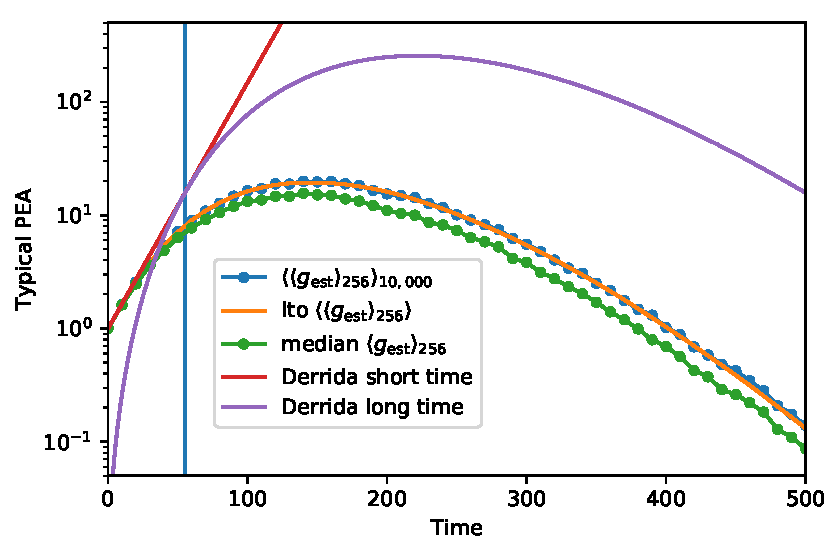
\includegraphics[height=9.3cm]{./chapter_people/figs/PEA.pdf}
\caption{Lines are obtained by exponentiating the various exponential 
growth rates. {\bf \underline{Blue line:}} $\ave{\ave{\gest}_{256}}_{10,000}$ is the numerical mean 
(approximation of the expectation value) 
over a super-ensemble of $S=10,000$ samples of $\gest$ estimated in sub-ensembles of $\N=256$ GBMs each. 
{\bf \underline{Green line:}} median in a super-ensemble of $S$ samples of $\gest$, each estimated in sub-ensembles of size $\N$. 
{\bf \underline{Yellow line:}} An exact expression for $d\ave{\ln\ave{\x}_\N}$, derived using \Ito calculus, see \cite{PetersAdamou2018b}. We evaluate the expression by Monte Carlo, and integrate, $\ave{\ln\ave{\x}_\N}=\int_{0}^{\t} d\ave{\ln\ave{\x}_\N}$. Exponentiation yields the yellow line. 
{\bf \underline{Red line:}} short-time behavior, based on the random energy model, \eref{gest_7}.
{\bf \underline{Purple line:}} long-time behavior, based on the random energy model, \eref{gest_8}. {\bf \underline{Vertical line:}} Crossover between the regimes at $t_c=\frac{2\ln \N}{\gsigma^2}$, corresponding to $\beta_c=\frac{2(\ln 2)^{1/2}}{J}$.
{\bf \underline{Parameters:}} $\N=256$, $S=10,000$, $\gmu=0.05$, $\gsigma=\sqrt{0.2}$.}
\flabel{1}
\end{figure}
\FloatBarrier